\chapter{Resultados e Discussões}
\label{cap:resultados}

Este capítulo apresenta os achados empíricos do estudo, com foco na experiência do usuário medida por \textit{Core Web Vitals} (coleta em campo, no cliente) e, de forma complementar, em diagnósticos laboratoriais do Lighthouse. Como contexto operacional, reporta-se também o consumo de CPU, memória e PIDs dos contêineres durante as execuções. A metodologia, o ambiente controlado e os procedimentos de coleta já foram descritos no Cap.~\ref{cap:estudo_caso}; aqui concentramos a atenção em resultados e implicações.

\section{Resultados}
Os testes cobriram as duas variantes da WallTech (\acrshort{ssr}/\acrshort{mpa} em Next.js e \acrshort{csr}/\acrshort{spa} em React) nas páginas: inicial, resultados de busca e detalhes da notícia. Para cada cenário, foram realizados 10--15 carregamentos após \textit{warm-up}, e as leituras são analisadas por mediana (p50) e, quando pertinente, p95.

\subsubsection*{Fontes de dados}
\begin{itemize}
  \item \textbf{Web Vitals (núcleo)}: \acrshort{ttfb}, \acrshort{fcp}, \acrshort{lcp}, \acrshort{cls}, \acrshort{inp} registrados no cliente e persistidos em NDJSON.
  \item \textbf{Lighthouse (apoio)}: \textbf{TBT} e principais \textbf{oportunidades/auditorias} de desempenho, além de verificações de \textbf{Acessibilidade} e \textbf{SEO}.
  \item \textbf{Recursos do servidor}: CPU/memória/PIDs via \texttt{docker stats}, como contexto de custo de execução.
\end{itemize}

\subsubsection*{Metas de referência}
Adotaram-se os seguintes alvos para interpretação:
\begin{itemize}
  \item \textbf{LCP} $\leq 2{,}5$\,s;\quad \textbf{CLS} $\leq 0{,}10$;\quad \textbf{INP} $\leq 200$\,ms;\quad \textbf{TTFB} $\leq 800$\,ms.
  \item \textbf{TBT (Lighthouse)} $<200$\,ms;\quad \textbf{Acessibilidade (LH)} $\geq 90$;\quad \textbf{SEO (LH)} $\geq 90$.
\end{itemize}

\subsection{Resultados para SSR}
\label{subsec:resultados-ssr}

\subsubsection*{Recursos do servidor}
Ao longo dos cenários, o contêiner \textit{Next.js} manteve \textbf{CPU} baixa e estável (aprox.\ 8--13\%), sem picos relevantes; a queda ao final da série coincide com o término do experimento (\autoref{fig:ssr-cpu}). A \textbf{memória} permaneceu em patamar quase constante, com variação estreita e redução apenas no encerramento das execuções (\autoref{fig:ssr-mem}). Esse comportamento é compatível com o processamento por requisição do SSR e não sinaliza saturação.

\begin{figure}[H]
  \centering
  \caption{Média de uso de CPU por tempo (\acrshort{ssr})}
  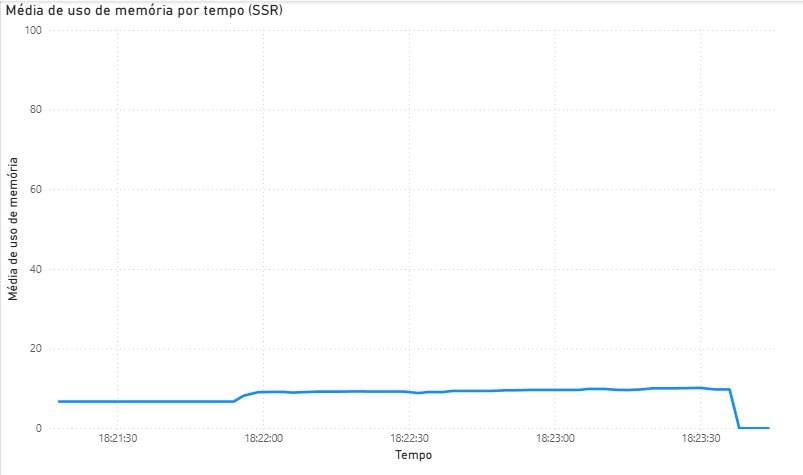
\includegraphics[width=0.9\textwidth]{media/uso_cpu_ssr.jpeg}
  \legend{Fonte: os autores.}
  \label{fig:ssr-cpu}
\end{figure}

\begin{figure}[H]
  \centering
  \caption{Média de uso de memória por tempo (\acrshort{ssr})}
  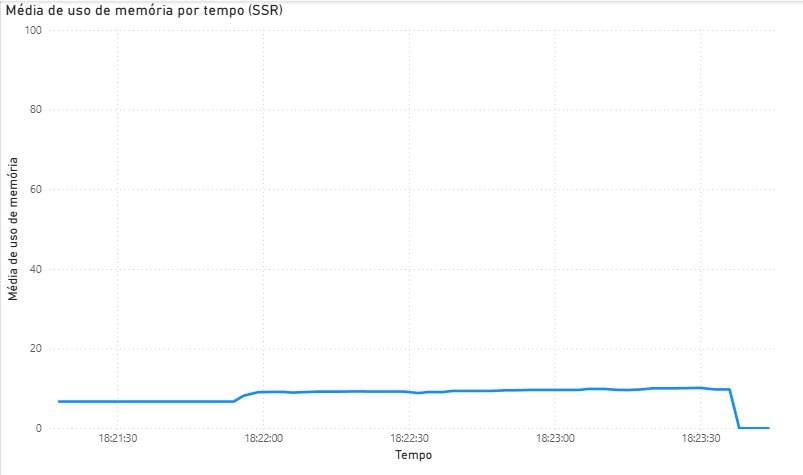
\includegraphics[width=0.9\textwidth]{media/uso_memoria_ssr.jpeg}
  \legend{Fonte: os autores.}
  \label{fig:ssr-mem}
\end{figure}

\subsubsection*{Web Vitals (cliente)}
Conforme a \autoref{fig:ssr-webvitals}, as leituras de campo foram, em sua maioria, classificadas como \textit{good}. Os poucos casos de \textit{needs-improvement} concentraram-se em \acrshort{lcp} e \acrshort{inp}, e houve uma fração reduzida de \acrshort{fcp} em \textit{poor} — efeito compatível com custos de \textit{hydration} e com elementos visuais de grande porte na dobra (imagens \emph{hero}). Em relação às metas adotadas, os resultados situam-se, em geral, próximos ou dentro dos limiares de referência: \acrshort{lcp} $\leq 2{,}5$\,s; \acrshort{cls} $\leq 0{,}10$; \acrshort{inp} $\leq 200$\,ms; \acrshort{ttfb} $\leq 800$\,ms.

\begin{figure}[H]
  \centering
  \caption{Classificação das métricas de desempenho (\acrshort{ssr}) com Web Vitals}
  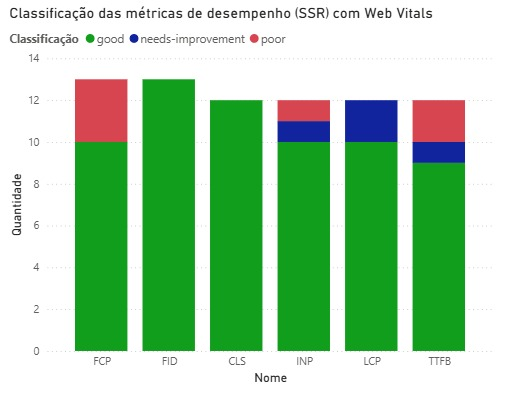
\includegraphics[width=0.9\textwidth]{media/metricas_ssr_web_vitals.jpeg}
  \legend{Fonte: os autores.}
  \label{fig:ssr-webvitals}
\end{figure}

\subsubsection*{Lighthouse (apoio diagnóstico)}
Para explicar variações residuais e priorizar melhorias, auditamos as rotas \emph{home}, \emph{busca} e \emph{detalhe} no modo \emph{Navigation} do Chrome DevTools, considerando três indicadores: \textbf{TBT}, \textbf{Acessibilidade} e \textbf{SEO}.
A Tabela~\ref{tab:lh-ssr} consolida as \textbf{medianas} observadas nos relatórios HTML anexados (\texttt{ssrMobile.html}, \texttt{ssrMobileBusca.html}, \texttt{ssrtestePage.html}).

\begin{table}[H]
\centering
\caption{Lighthouse (SSR) — mediana por rota}
\label{tab:lh-ssr}
\begin{tabular}{|l|c|c|c|}
\hline
\textbf{Rota} & \textbf{TBT (ms)} & \textbf{Acessibilidade (\%)} & \textbf{SEO (\%)} \\
\hline
Home    & 12 & 95  & 100 \\
Busca   & 10 & 99  & 100 \\
Detalhe & 0--7\footnotemark[1] & 100 & 100 \\
\hline
\end{tabular}
\end{table}
\footnotetext[1]{Variações muito baixas entre execuções; mediana $\approx$ 5\,ms.}

\noindent \textit{Leitura.}
(i) \textbf{TBT} muito abaixo da meta interna ($<200$\,ms) em todas as rotas, corroborando \acrshort{inp} em \textit{good};
(ii) \textbf{Acessibilidade} alta (95--100\%), com ajustes residuais (hierarquia de headings, foco visível, rótulos) de fácil endereçamento;
(iii) \textbf{SEO} consistente (100\%), indicando sinalização adequada (título, \emph{meta description}, \texttt{canonical}, \texttt{robots}, \texttt{viewport}) — aspecto particularmente relevante no fluxo SSR.

\subsubsection*{Síntese (SSR)}
Servidor com CPU/RAM contidos; \emph{Web Vitals} majoritariamente \textit{good}, com atenção pontual a \acrshort{lcp}/\acrshort{fcp} em páginas com imagens destacadas e pós-hidratação; \emph{Lighthouse} confirma \textbf{TBT} reduzido e \textbf{altos escores} de \textbf{Acessibilidade} e \textbf{SEO}, sustentando o SSR para páginas públicas sensíveis à descoberta.




\subsection{Resultados para CSR}
\label{subsec:resultados-csr}

\subsubsection*{Recursos do servidor}
O contêiner da \emph{SPA} apresentou \textbf{CPU} muito baixa e estável, com oscilações discretas e picos inferiores a 5\% (\autoref{fig:csr-cpu}). A \textbf{memória} permaneceu praticamente constante e em patamar reduzido durante todo o ensaio, coerente com a entrega estática e a execução da lógica no cliente (\autoref{fig:csr-mem}). Não se observaram sinais de saturação.

\begin{figure}[H]
\centering
\caption{Média de uso de CPU por tempo (\acrshort{csr})}
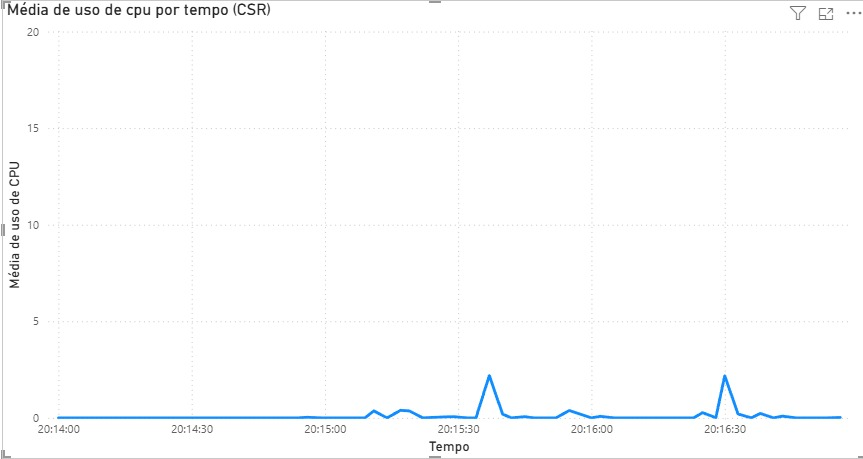
\includegraphics[width=0.9\textwidth]{media/uso_cpu_csr.jpeg}
\legend{Fonte: os autores.}
\label{fig:csr-cpu}
\end{figure}

\begin{figure}[H]
\centering
\caption{Média de uso de memória por tempo (\acrshort{csr})}
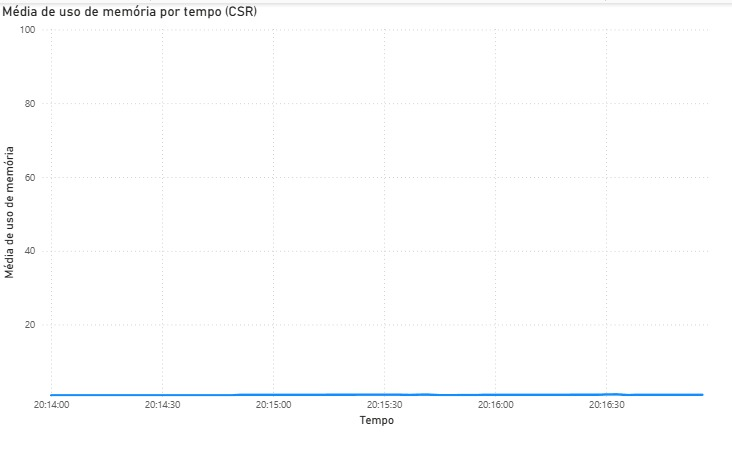
\includegraphics[width=0.9\textwidth]{media/uso_memoria_csr.jpeg}
\legend{Fonte: os autores.}
\label{fig:csr-mem}
\end{figure}

\subsubsection*{Web Vitals (cliente)}
As leituras de campo indicam \textbf{predomínio de \textit{good}} em \acrshort{ttfb}, \acrshort{fcp}, \acrshort{lcp} e \acrshort{inp} (\autoref{fig:csr-webvitals}). O ponto fora da curva é a \textbf{\acrshort{cls}}, com concentrações em \textit{poor}. O padrão é típico de SPAs quando ocorrem \emph{layout shifts} durante a hidratação ou quando imagens/slots não reservam espaço antes do carregamento (dimensões ausentes, fontes sem \emph{preload}, inserções acima da dobra). Em relação às metas, as leituras ficaram, em geral, dentro ou próximas dos limiares de referência (\acrshort{lcp} $\leq 2{,}5$\,s; \acrshort{cls} $\leq 0{,}10$; \acrshort{inp} $\leq 200$\,ms; \acrshort{ttfb} $\leq 800$\,ms), com a ressalva da \acrshort{cls}.

\begin{figure}[H]
\centering
\caption{Classificação das métricas de desempenho (\acrshort{csr}) com Web Vitals}
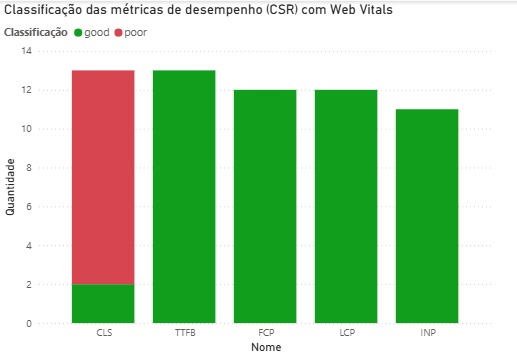
\includegraphics[width=0.9\textwidth]{media/metricas_csr_web_vitals.jpeg}
\legend{Fonte: os autores.}
\label{fig:csr-webvitals}
\end{figure}

\subsubsection*{Lighthouse (apoio diagnóstico)}
Para explicar oscilações residuais e orientar priorizações, auditamos as rotas críticas no \emph{Chrome DevTools} (modo \emph{Navigation}), com três indicadores: \textbf{TBT}, \textbf{Acessibilidade} e \textbf{SEO}.

\noindent \textit{Achados.}
\begin{itemize}
  \item \textbf{TBT}: manteve-se em patamar \textbf{muito baixo} (dezenas de milissegundos) nas páginas inspecionadas, consistente com \acrshort{inp} \textit{good}.
  \item \textbf{Acessibilidade}: escores altos na \emph{home} (93--94\,\%), com ajustes residuais (hierarquia de \emph{headings}, foco visível, rótulos/\textit{alt}) — valores observados nos relatórios “Home (Web)” e “Home (Mobile)”.
  \item \textbf{SEO}: a \emph{home} registrou \textasciitilde{}83\,\% (Web e Mobile), sugerindo oportunidades pontuais (por exemplo, \emph{meta description}/\texttt{canonical}/\texttt{robots}/\texttt{hreflang}, quando aplicável).
\end{itemize}

\noindent \textit{Leitura.} Em conjunto, os relatórios apontam que o gargalo do \textbf{CSR} não está em bloqueio de \emph{main thread} (TBT baixo), mas em \textbf{estabilidade visual} e em alguns sinais de \textbf{SEO}. Na prática, os seguintes ajustes tendem a capturar os ganhos: (i) reservar dimensões de imagens e \emph{cards} acima da dobra (\texttt{width}/\texttt{height} ou \texttt{aspect-ratio}); (ii) \emph{preload} de fontes e imagens \emph{hero} (com \texttt{font-display: swap}); (iii) evitar inserções DOM acima da dobra durante a hidratação; (iv) completar metadados de SEO (título/descrição/\texttt{canonical}/\texttt{robots}) e revisar indexabilidade.

\subsubsection*{Síntese (CSR)}
Servidor praticamente ocioso (CPU e RAM baixos); \emph{Web Vitals} em boa forma para \acrshort{ttfb}/\acrshort{fcp}/\acrshort{lcp}/\acrshort{inp}, com atenção especial à \textbf{\acrshort{cls}}. O \emph{Lighthouse} confirmou \textbf{TBT reduzido}, \textbf{Acessibilidade} alta e \textbf{SEO} com melhorias de rápida implementação, coerentes com o perfil de \textbf{SPA} e suas responsabilidades no cliente.

\subsection{Comparação entre SSR e CSR}
\label{subsec:comparacao-ssr-csr}

Esta seção compara, de forma integrada, experiência do usuário (\emph{Web Vitals} em campo), diagnóstico laboratorial (Lighthouse: TBT, Acessibilidade e SEO) e custo operacional (CPU/Memória nos contêineres). A leitura está ancorada nas medianas (p50) e, quando pertinente, no p95 dos cenários \textbf{home}, \textbf{busca} e \textbf{detalhe}.

\begin{table}[H]
\centering
\caption{Síntese comparativa dos resultados (SSR $\times$ CSR) neste estudo}
\label{tab:comparativo-ssr-csr}
\begin{tabular}{|p{4.2cm}|p{5.2cm}|p{5.2cm}|}
\hline
\textbf{Aspecto} & \textbf{SSR (MPA/Next.js)} & \textbf{CSR (SPA/React)} \\
\hline
\textbf{CPU no servidor} & Baixa e estável (\textit{$\sim$8--13\%}), sem picos relevantes. & Muito baixa; oscilações discretas com picos $<5\%$. \\
\hline
\textbf{Memória no servidor} & Estável, variação estreita; queda apenas ao término dos testes. & Muito baixa e praticamente constante. \\
\hline
\textbf{Web Vitals (campo)} & Predominância de \textit{good}; pequenos trechos \textit{needs-improvement} em \textbf{LCP}/\textbf{INP} e fração \textit{poor} em \textbf{FCP} (páginas com imagens \emph{hero} e pós-hidratação). & \textbf{TTFB}/\textbf{FCP}/\textbf{LCP}/\textbf{INP} majoritariamente \textit{good}; \textbf{CLS} com ocorrências \textit{poor} (shifts na montagem/hidratação e elementos sem reserva de espaço). \\
\hline
\textbf{Lighthouse: TBT} & \textbf{Muito baixo} (home $\approx$12\,ms; busca $\approx$10\,ms; detalhe $\approx$5\,ms). & \textbf{Muito baixo} (ordem de dezenas de ms na home). \\
\hline
\textbf{Lighthouse: Acessibilidade} & \textbf{Alta} (95--100\%). & \textbf{Alta} (93--94\% na home). \\
\hline
\textbf{Lighthouse: SEO} & \textbf{100\%} nas rotas auditadas. & \textbf{$\sim$83\%} na home; indica metadados/sinalizações a completar. \\
\hline
\textbf{Leitura operacional} & Parte da renderização no servidor melhora \textbf{TTFB}/\emph{first paint} e favorece \textbf{SEO}; cuidado com \emph{hydration} e imagens de grande porte. & Renderização no cliente alivia o servidor e mantém \textbf{TBT/INP} baixos; requer disciplina de layout para evitar \textbf{CLS} e ajustes de \textbf{SEO}. \\
\hline
\end{tabular}
\end{table}

\subsubsection{Pontos fortes do SSR.}
(i) \textbf{Tempo até primeira resposta/primeiro conteúdo.} O HTML pré-renderizado reduz o tempo de exibição inicial, o que se refletiu em \textit{TTFB}/\textit{FCP} consistentes e \textbf{TBT} residual nas auditorias.  
(ii) \textbf{Descoberta e rastreabilidade.} \textbf{SEO} com 100\% nas rotas testadas, reforçando a adequação do SSR para páginas públicas e conteúdo editorial.  
(iii) \textbf{Acessibilidade.} Escores elevados (95--100\%) indicam que a estrutura entregue pelo servidor chega semanticamente “pronta” ao cliente.  
(iv) \textbf{Previsibilidade de performance.} Em cenários com rede/CPU do cliente mais limitados, a renderização no servidor reduz o risco de longas tarefas no \emph{main thread} do navegador.

\subsubsection{Pontos fracos do SSR.}
(i) \textbf{Custo de hidratação.} Após o HTML inicial, a ativação dos componentes pode degradar \textbf{LCP}/\textbf{FCP} em páginas com imagens \emph{hero} e muito JS.  
(ii) \textbf{Custo no servidor (ainda que baixo).} O processamento por requisição eleva discretamente \textbf{CPU}/\textbf{memória} no host frente ao CSR.  
(iii) \textbf{Complexidade de build/deploy.} Estratégias como \emph{streaming}, \emph{partial/targeted hydration} e \emph{Server Components} elevam a complexidade de arquitetura.

\subsubsection{Pontos fortes do CSR.}
(i) \textbf{Interatividade contínua.} Navegação sem recarregar página, com \textbf{TBT/INP} baixos nas auditorias e nos dados de campo.  
(ii) \textbf{Custo operacional.} \textbf{CPU/memória} do servidor permanecem muito baixos: entrega estática + execução no cliente.  
(iii) \textbf{Escalabilidade horizontal simples.} Conteúdo estático facilita cache/CDN, reduzindo pressão no backend.

\subsubsection{Pontos fracos do CSR.}
(i) \textbf{Estabilidade visual.} \textbf{CLS} apresentou ocorrências \textit{poor}; o risco de \emph{layout shifts} aumenta quando não há reserva de espaço para mídia e quando há inserções acima da dobra na hidratação.  
(ii) \textbf{Sinais de SEO.} Escores \textasciitilde83\% na home (Lighthouse) indicam metadados/sinalizações a completar (p.\,ex., \emph{meta description}, \texttt{rel=canonical}, \texttt{robots}, \texttt{hreflang} quando aplicável).  
(iii) \textbf{Dependência de JS no cliente.} Em dispositivos muito modestos, o custo de montar a aplicação pode afetar \textit{FCP}/\textit{LCP} se o \emph{bundle} não for estritamente otimizado.

\subsection{Discussão}
\label{subsec:discussao-comparativa}
\textbf{(i) Recursos do servidor.} O \acrshort{ssr} consumiu levemente mais \textbf{CPU/memória} (ainda baixos) do que o \acrshort{csr}, resultado esperado do processamento por requisição. O \acrshort{csr}, por sua vez, opera praticamente como \emph{static hosting}, com custo mínimo no host. \\
\textbf{(ii) Experiência do usuário.} Em \acrshort{ssr}, a entrega inicial é perceptivelmente rápida e os escores de \textbf{SEO} e \textbf{Acessibilidade} são superiores; as pequenas perdas em \textbf{LCP}/\textbf{FCP} aparecem em páginas com imagens grandes e após a hidratação. Em \acrshort{csr}, \textbf{TTFB}/\textbf{FCP}/\textbf{LCP}/\textbf{INP} resultaram majoritariamente \textit{good}, e o \textbf{TBT} foi baixo; o principal cuidado é a \textbf{CLS}. \\
\textbf{(iii) Coerência entre campo e laboratório.} Os \textit{Web Vitals} em campo (usuário real) e o \textbf{TBT} do Lighthouse (laboratório) convergiram: baixo bloqueio de \emph{main thread} nos dois modelos. As divergências localizam-se em \textbf{CLS} (CSR) e \textbf{SEO} (CSR $<$ SSR), que são áreas classicamente sensíveis à estratégia de renderização.

\subsection{Implicações práticas}
\begin{itemize}
  \item \textbf{Priorizar SSR} quando: páginas públicas dependentes de \textbf{SEO}, conteúdo editorial/comercial, catálogos indexáveis e cenários em que \textbf{TTFB} e \textbf{exibição inicial} são críticos para engajamento e descoberta.
  \item \textbf{Priorizar CSR} quando: aplicações altamente interativas (dashboards, sistemas internos), requisitos fortes de navegação fluida no cliente e \textbf{custo de servidor} deve permanecer mínimo.
\end{itemize}

\subsection{Ajustes recomendados}
\textbf{SSR (mitigar LCP/INP).} Otimizar e dimensionar imagens (usar \texttt{priority} para \emph{hero} e \emph{lazy} abaixo da dobra), considerar \emph{streaming}/\emph{partial hydration}/\emph{Server Components}, reduzir JS não crítico e declarar \texttt{preload}/\texttt{dns-prefetch} para recursos essenciais. \\
\textbf{CSR (mitigar CLS e elevar SEO).} Reservar dimensões de mídia (\texttt{width}/\texttt{height} ou \texttt{aspect-ratio}); evitar inserções acima da dobra durante a hidratação; \texttt{font-display: swap} com \emph{preload} de fontes e imagens \emph{hero}; placeholders do tamanho final; completar metadados e sinalizações (\emph{title}/\emph{description}/\texttt{canonical}/\texttt{robots}/\texttt{hreflang} quando aplicável).

\subsection{Síntese}
No cenário testado, \textbf{SSR} e \textbf{CSR} entregaram boa experiência de uso com \textbf{baixa pressão de recursos}. O \textbf{SSR} destacou-se por \textbf{SEO} e \textbf{exibição inicial} mais previsível; o \textbf{CSR} reduziu o \textbf{custo no servidor} e manteve \textbf{TBT/INP} baixos, com a contrapartida de maior propensão a \textbf{CLS} e sinais de \textbf{SEO} a complementar. A decisão deve considerar \textbf{perfil de tráfego}, \textbf{exigência de descoberta} e \textbf{tipo de interação}, aplicando as otimizações para mitigar os pontos fracos identificados em cada abordagem.
